\cleardoublepage\phantomsection
\phantomsection\mtcaddchapter[Anexo A: información suplementaria]
\FormatoAnexoA

%Agrego las marcas laterales
\AddLabelsAxUno

%Problemas con el tema del fancystyle
\let\originalstyle=\thispagestyle            % Store the command for later reuse.
\def\thispagestyle#1{\fancyfoot[C]{}}       % This clears footer in the center if fancyhdr is in use.
\def\thispagestyle#1{\originalstyle{empty}} % Use this to get blank header+footer, TeXnically it is only \thispagestyle{empty}.
\def\thispagestyle#1{}                       % This line completely ignores the content of the \thispagestyle command.

%Esto cambia el contador de las figuras para que coloque la letra del apéndice
\renewcommand\thefigure{A.\arabic{figure}} 

%Nombre del Anexo
\chapter*{Anexo A: información suplementaria}
    
    Se agregan en éste anexo los gráficos, imágenes y espectros complementarios que fueron apartados del cuerpo principal de la tesis. 
    %por motivos de de favilitar la lectuta

    \subsection*{Figuras correspondientes al capítulo \ref{chap:Mesoporosos}}

    %Simplificado
      %\subsubsection*{Método simplificado}

     %Microscopia F127 Simplificado
         \begin{figure}[th!]          
 	   	    \begin{subfigure}{0.495\textwidth}
	       	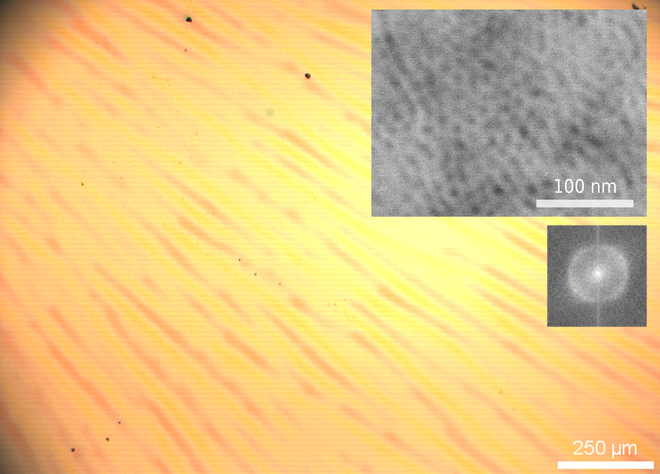
\includegraphics[width=\textwidth]{Imagenes/Au_EtF127-Combinada.jpg}
	   		\end{subfigure}
	   		\begin{subfigure}{0.495\textwidth}
	   	    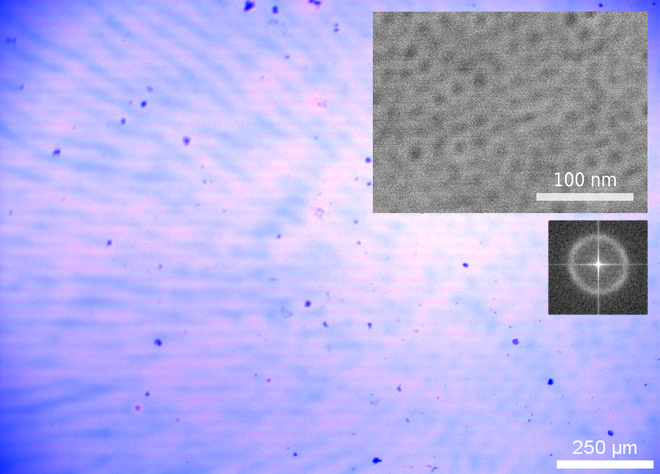
\includegraphics[width=\textwidth]{Imagenes/Si_EtF127-Combinada.jpg}
	   		\end{subfigure}
			 \caption[Microscopías \pdmF\space tratamiento simplificado.]{Microscopías ópticas para Sim\pdmF. Izquierda: sobre sustrato de Au. Derecha: sobre sustrato de Si. En los respectivos recuadros se observa el detalle por MEB junto a la transformada de Fourier del arreglo nanoporoso.}
			 \label{fig:Microscopia_F127_simplificado}	
		    % \end{figure}		
	 		\vspace*{1cm}
	 %Microscopia CTAB Simplificado
	     %\begin{figure}
 	   	    \begin{subfigure}{0.495\textwidth}
	       	\includegraphics[width=\textwidth]{Imagenes/Au_EtCTAB-Combinada.jpg}
	   		\end{subfigure}
	   		\begin{subfigure}{0.495\textwidth}
	   	    \includegraphics[width=\textwidth]{Imagenes/Si_EtCTAB-Combinada.jpg}
	   		\end{subfigure}
			 \caption[Microscopías \pdmC\space tratamiento simplificado.]{Microscopías ópticas para Sim\pdmC. Obsérvese las grietas presentes cuando se sintetiza sobre Au (izquierda), mientras que sobre Si las Sim\pdmC\space no presentan rupturas ni discontinuidades.}
			 \label{fig:Microscopia_CTAB_simplificado}	
		     \end{figure}	
		
	 %Elipso F127 Simplificaco	     
	  	 \begin{figure}
			  	\begin{subfigure}{0.495\textwidth}
			  	\includegraphics[width=\textwidth]{Graficos/SI_F127_simplificado_EPA.pdf}
				\caption{Isorterma de adsorción/desorción de agua realizada por PEA para una Sim\pdmF.}
				\label{fig:F127_simplificado_EPA}
				\end{subfigure}
				\begin{subfigure}{0.495\textwidth}
			  	\includegraphics[width=\textwidth]{Graficos/SI_F127_simplificado_PSD.pdf}
				\caption{Distribución de tamaño de poro y cuello.\\ }
				\label{fig:F127_simplificado_PSD}
				\end{subfigure}
				\caption[Elipsoporosimetría \pdmF\space tratamiento simplificado.]{Resultados de elipsoporosimetría ambiental para una Sim\pdmF\space.}
				\label{fig:F127_simplificado}
				\end{figure}
	
	 %Elipso CTAB Simplificad
		  \begin{figure}	
			\begin{subfigure}{0.495\textwidth}
		  	\includegraphics[width=\textwidth]{Graficos/SI_CTAB_simplificado_EPA.pdf}
			\caption{Isorterma de adosroción/desorción de agua ralizada por PEA para una Sim\pdmC.}
			\label{fig:CTAB_simplificado_EPA}
			\end{subfigure}
			\begin{subfigure}{0.495\textwidth}
		  	\includegraphics[width=\textwidth]{Graficos/SI_CTAB_simplificado_PSD.pdf}
			\caption{Distribución de tamaño de poro y cuello.\\ }
			\label{fig:CTAB_simplificado_PSD}
			\end{subfigure}
			\caption[Elipsoporosimetría \pdmC\space tratamiento simplificado.]{Resultados de elipsoporosimetría ambiental para una Sim\pdmC.}
			\end{figure}			

	 %FTIR Simplificado		
	
		 \begin{figure}
				\centering
				\includegraphics[width=0.75\textwidth]{Graficos/IR_F127_simplificado.pdf}
				\caption[FTIR \pdmF\space tratamiento simplificado.]{Espectro de absorción en el IR para una Sim\pdmF\space sintetizada con el tratamiento simplificado antes y después de extraer el surfactante. Desaparece la banda de estiramiento C-H correspondiente al surfactante luego de la extracción.}
				\label{fig:IR_F127_simplificado}
				\end{figure}
			
	 %FTIR Simplificado
	  
	      \begin{figure}
			\centering
			\includegraphics[width=0.75\textwidth]{Graficos/IR_CTAB_simplificado.pdf}
			\caption[FTIR \pdmC\space tratamiento simplificado.]{Espectro de absorción en el IR para una Sim\pdmC\space sintetizada con el tratamiento simplificado antes y después de extraer el surfactante. Todavía se puede apreciar un cantidad pequeña de surfactante luego de la extracción.}
			\label{fig:IR_CTAB_simplificado}
			\end{figure}	

	%Prolongado
		%\subsubsection*{Método prolongado}

		%Microscopia F127 Prolongado
			 \begin{figure}
		 	   	    \begin{subfigure}{0.495\textwidth}
			       	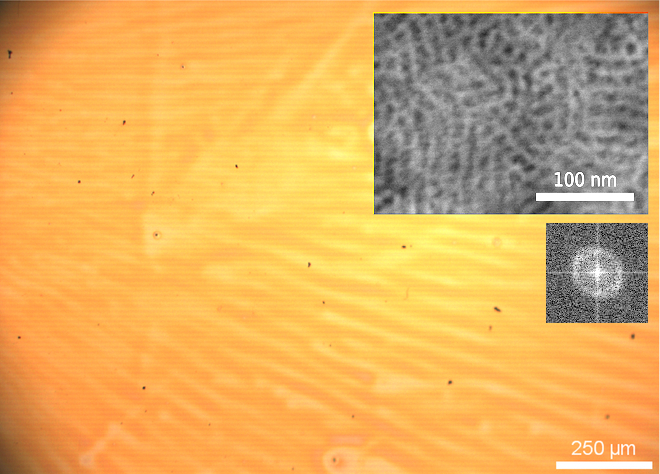
\includegraphics[width=\textwidth]{Imagenes/Au_130F127-Combinada.jpg}
			   		\end{subfigure}
			   		\begin{subfigure}{0.495\textwidth}
			   	    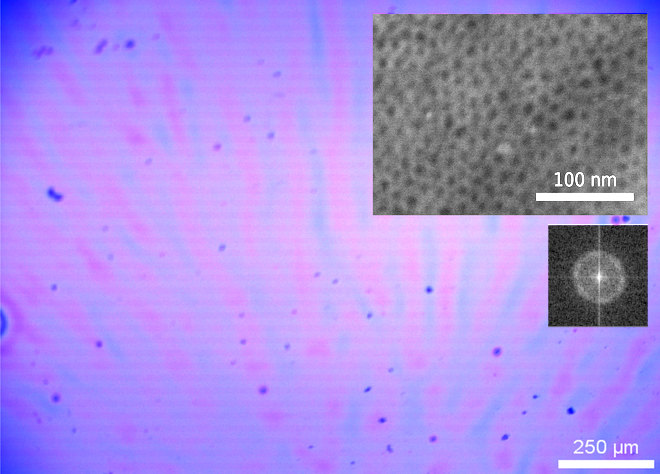
\includegraphics[width=\textwidth]{Imagenes/Si_130F127-Combinada.jpg}
			   		\end{subfigure}
					 \caption[Microscopía \pdmF\space tratamiento prolongado.]{Microscopías ópticas para Pro\pdmF. Izquierda: sobre sustrato de Au. Derecha: sobre sustrato de Si. En los respectivos recuadros se observa el detalle por MEB junto a la transformada de Fourier del arreglo nanoporoso.}
					 \label{fig:Microscopia_F127_prolongado}	
				     \end{figure}	

		%Microscopia CTAB Prolongado
		 \begin{figure}
	 	   	    \begin{subfigure}{0.495\textwidth}
		       	\includegraphics[width=\textwidth]{Imagenes/Au_130CTAB-Combinada.jpg}
		   		\end{subfigure}
		   		\begin{subfigure}{0.495\textwidth}
		   	    \includegraphics[width=\textwidth]{Imagenes/Si_130CTAB-Combinada.jpg}
		   		\end{subfigure}
				 \caption[Microscopía óptica \pdmC\space tratamiento prolongado.]{Microscopías ópticas para Pro\pdmC. Derecha: sobre sustrato de Au. Izquierda: sobre sustrato de Si.}
				 \label{fig:Microscopia_CTAB_prolongado}	
			     \end{figure}
			    
		%Elipso F127 Prolongado

			 \begin{figure}
			  	\begin{subfigure}{0.495\textwidth}
			  	\includegraphics[width=\textwidth]{Graficos/SI_F127_prolongado_EPA.pdf}
				\caption{Isoterma de adsorción/desorción de agua realizada por PEA para Pro\pdmF.}
				\label{fig:F127_prolongado_EPA}
				\end{subfigure}
				\begin{subfigure}{0.495\textwidth}
			  	\includegraphics[width=\textwidth]{Graficos/SI_F127_prolongado_PSD.pdf}
				\caption{Distribución de tamaño de poro y cuello.\\ }
				\label{fig:F127_prolongado_PSD}
				\end{subfigure}
				\caption[Elipsoporosimetría \pdmF\space tratamiento prolongado.]{Resultados de PEA para sistema Pro\pdmF\space sintetizada por el tratamientos prolongado, consistente en estabilización en humedad seguido de condensación por 7 días a \SI{130}{\celsius} y extracción.}
		 		\end{figure}

		%Elipso CTAB Prolongado
		 \begin{figure}
		  	\begin{subfigure}{0.495\textwidth}
		  	\includegraphics[width=\textwidth]{Graficos/SI_CTAB_prolongado_EPA.pdf}
			\caption{Isoterma de adosroción/desorción de agua ralizada por PEA para Pro\pdmC\space.}
			\label{fig:CTAB_prolongado_EPA}
			\end{subfigure}
			\begin{subfigure}{0.495\textwidth}
		  	\includegraphics[width=\textwidth]{Graficos/SI_CTAB_prolongado_PSD.pdf}
			\caption{Distribución de tamaño de poro y cuello.\\ }
			\label{fig:CTAB_prolongado_PSD}
			\end{subfigure}
			\caption[Elipsoporosimetría \pdmC\space tratamiento prolongado.]{Resultados de PEA para sistema Pro\pdmC\space sintetizada por el tratamientos prolongado, consistente en estabilización en humedad seguido de condensación por 7 días a \SI{130}{\celsius} y extracción.}
			\end{figure}

		%FTIR F127 Prolongado
	
	  \begin{figure}
			\centering
			\includegraphics[width=0.75\textwidth]{Graficos/IR_F127_prolongado.pdf}
			\caption[FTIR \pdmF\space tratamiento prolongado.]{Espectro de absorción de IR correspondiente a una Pro\pdmF\space antes y después de la extracción con 2-propanol.}
			\label{fig:IR_F127_prolongado}
			\end{figure}

		%FTIR CTAB Prolongado	
		\begin{figure}
			\centering
			\includegraphics[width=0.75\textwidth]{Graficos/IR_CTAB_prolongado.pdf}
			\caption[FTIR \pdmC\space tratamiento prolongado.]{Espectro de absorción de IR correspondiente a una Pro\pdmC\space  antes y después de la extracción con 2-propanol.}
			\label{fig:IR_CTAB_prolongado}
			\end{figure}		

	%Vacio
		%\subsubsection*{Método de alto vacío}

		%Microscopias F127
		 \begin{figure}
	 	   	    \begin{subfigure}{0.495\textwidth}
		       	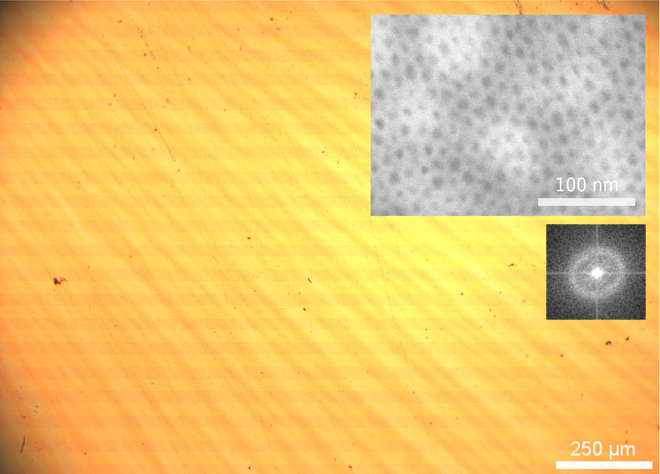
\includegraphics[width=\textwidth]{Imagenes/Au_130VF127-Combinada.jpg}
		   		\end{subfigure}
		   		\begin{subfigure}{0.495\textwidth}
		   	    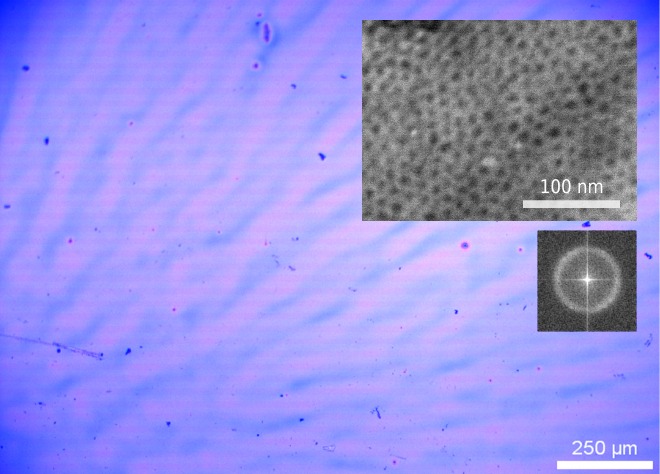
\includegraphics[width=\textwidth]{Imagenes/Si_130VF127-Combinada.jpg}
		   		\end{subfigure}
				 \caption[Microscopía óptica \pdmF\space tratamiento vacío.]{Microscopías ópticas para Vac\pdmF. Izquierda: sobre sustrato de Au. Derecha: sobre sustrato de Si. En los respectivos recuadros se observa el detalle por MEB junto a la transformada de Fourier del arreglo nanoporoso.}
				 \label{fig:Microscopia_F127_vacio}	
			     \end{figure}	

		%Microscopias CTAB
		 \begin{figure}
		 	   	    \begin{subfigure}{0.495\textwidth}
			       	\includegraphics[width=\textwidth]{Imagenes/Au_130VCTAB-Combinada.jpg}
			   		\end{subfigure}
			   		\begin{subfigure}{0.495\textwidth}
			   	    \includegraphics[width=\textwidth]{Imagenes/Si_130VCTAB-Combinada.jpg}
			   		\end{subfigure}
					 \caption[Microscopía óptica \pdmC\space tratamiento vacío.]{Microscopías ópticas para Vac\pdmC. Izquierda: sobre sustrato de Au. Derecha: sobre sustrato de Si.}
					 \label{fig:Microscopia_CTAB_vacio}	
				     \end{figure}		 	    

		%Microscopias Mixtos
		  \begin{figure}
		 	   	    \begin{subfigure}{0.495\textwidth}
			       	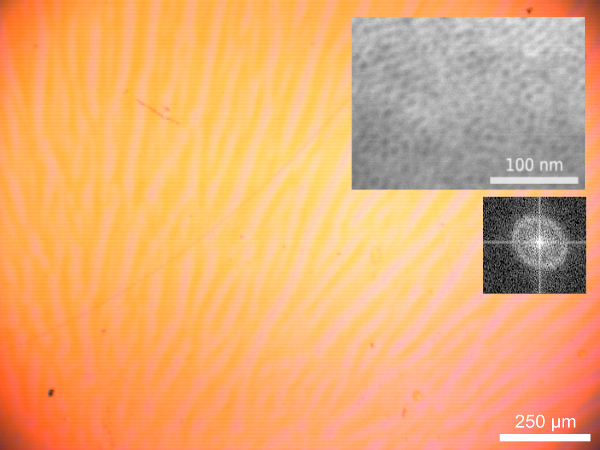
\includegraphics[width=\textwidth]{Imagenes/Au_SZF-Vacio.jpg}
			   		\end{subfigure}
			   		\begin{subfigure}{0.495\textwidth}
			   	    \includegraphics[width=\textwidth]{Imagenes/Au_SZB-Vacio.jpg}
			   		\end{subfigure}
					 \caption[Microscopía óptica \pdm\space mixtas Zr/Si.]{Microscopías ópticas para Vac\pdmZ\space depositadas sobre electrodos de Au. Izquierda: Utilizando F127 como surfactante. Derecha: Utilizando Brij58 como surfactante.}
					 \label{fig:Microscopia_ZrSi_vacio}	
				     \end{figure}

		%Elipso F127
		   \begin{figure}
			  	\begin{subfigure}{0.495\textwidth}
			  	\includegraphics[width=\textwidth]{Graficos/SI_F127_vacio_EPA.pdf}
				\caption{Elipsoporosimetría de una \pdmF\space tratamiento 7 días en alto vacío.}
				\label{fig:F127_vacio_EPA}
				\end{subfigure}
				\begin{subfigure}{0.495\textwidth}
			  	\includegraphics[width=\textwidth]{Graficos/SI_F127_vacio_PSD.pdf}
				\caption{Distribución de tamaño de poro y cuello.\\ }
				\label{fig:F127_vacio_PSD}
				\end{subfigure}
				\caption[Elipsoporosimetría \pdmF\space tratamiento alto vacío.]{Resultados de elipsoporosimetría ambiental para una Vac\pdmF, 7 días a \SI{130}{\celsius} en alto vacío (P=\SI{1e-5}{\milli\bar}).}
				\end{figure}
		
		%Elipso CTAB
		  \begin{figure}
		  	\begin{subfigure}{0.495\textwidth}
		  	\includegraphics[width=\textwidth]{Graficos/SI_CTAB_vacio_EPA.pdf}
			\caption{Elipsoporsimetría de una \pdmC\space Tratamiento 7 días alto vacío.}
			\label{fig:CTAB_vacio_EPA}
			\end{subfigure}
			\begin{subfigure}{0.495\textwidth}
		  	\includegraphics[width=\textwidth]{Graficos/SI_CTAB_vacio_PSD.pdf}
			\caption{Distribución de tamaño de poro y cuello.\\ }
			\label{fig:CTAB_vacio_PSD}
			\end{subfigure}
			\caption[Elipsoporosimetría \pdmC\space tratamiento alto vacío.]{Resultados de elipsoporosimetría ambiental para una Vac\pdmC, 7 días a \SI{130}{\celsius} en alto vacío (P=\SI{1e-5}{\milli\bar}).}
			\end{figure} 	
		
		%FTIR F127
         \begin{figure}
			 	\centering
			 	\includegraphics[width=0.75\textwidth]{Graficos/IR_F127_vacio.pdf}
			 	\caption[FTIR \pdmF\space tratamiento prolongado.]{Espectro de absorción de IR correspondiente a una Vac\pdmF, antes y después de la extracción con 2-propanol.}
			 	\label{fig:IR_F127_vacio}
			    \end{figure}
					
		%FTIR CTAB
		 \begin{figure}
			 	\centering
			 	\includegraphics[width=0.75\textwidth]{Graficos/IR_CTAB_vacio.pdf}
			 	\caption[FTIR \pdmC\space tratamiento prolongado.]{Espectro de absorción de IR correspondiente a una Vac\pdmC, antes y después de la extracción con 2-propanol.}
			 	\label{fig:IR_CTAB_vacio}
			 	\end{figure}

    %Ácido
    	
    	%\subsubsection*{Método ácido}
    	
    	%Microscopia F127
     	     \begin{figure}
	 	   	    \begin{subfigure}{0.495\textwidth}
		       	\includegraphics[width=\textwidth]{Imagenes/Au_AF127-Combinada.jpg}
		   		\end{subfigure}
		   		\begin{subfigure}{0.495\textwidth}
		   	    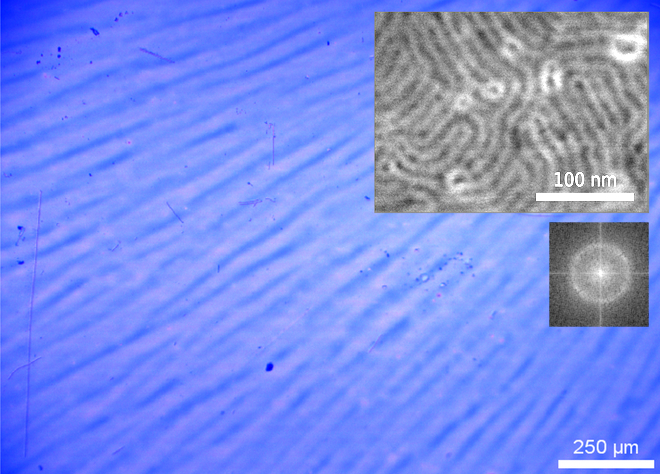
\includegraphics[width=\textwidth]{Imagenes/Si_AF127-Combinada.jpg}
		   		\end{subfigure}
				 \caption[Microscopía óptica \pdmF tratamiento en medio ácido.]{Microscopías ópticas para Áci\pdmF. Izquierda: sobre sustrato de Au. Derecha: sobre sustrato de Si. En los respectivos recuadros se observa el detalle por MEB junto a la transformada de Fourier (sobre silicio) del arreglo nanoporoso.}
				 \label{fig:Microscopia_F127_acido}	
			     \end{figure}
   		
   		%Microscopia CTAB
   			\begin{figure}
 	   	    \begin{subfigure}{0.495\textwidth}
	       	\includegraphics[width=\textwidth]{Imagenes/Au_ACTAB-Combinada.jpg}
	   		\end{subfigure}
	   		\begin{subfigure}{0.495\textwidth}
	   	    \includegraphics[width=\textwidth]{Imagenes/Si_ACTAB-Combinada.jpg}
	   		\end{subfigure}
			 \caption[Microscopía óptica \pdmC tratamiento en medio ácido.]{Microscopías ópticas para Áci\pdmC. Izquierda: sobre sustrato de Au. Derecha: sobre sustrato de Si.}
			 \label{fig:Microscopia_CTAB_acido}	
		     \end{figure}
   	
		%Elipso F127

		    \begin{figure}
		  	\begin{subfigure}{0.495\textwidth}
		  	\includegraphics[width=\textwidth]{Graficos/SI_F127_acido_EPA.pdf}
			\caption{Isoterma de adsorción/desorción de agua realizada por PEA para una Áci\pdmF.}
			\label{fig:F127_acido_EPA}
			\end{subfigure}
			\begin{subfigure}{0.495\textwidth}
		  	\includegraphics[width=\textwidth]{Graficos/SI_F127_acido_PSD.pdf}
			\caption{Distribución de tamaño de poro y cuello.\\ }
			\label{fig:F127_acido_PSD}
			\end{subfigure}
			\caption[Elipsoporosimetría \pdmF\space tratamiento ácido.]{Resultados de elipsoporosimetría ambiental para una Áci\pdmF.}
			\end{figure}     

		%Elipso CTAB
		
			\begin{figure}
		  	\begin{subfigure}{0.495\textwidth}
		  	\includegraphics[width=\textwidth]{Graficos/SI_CTAB_acido_EPA.pdf}
			\caption[Elipsoporsimetría \pdmC\space tratamiento ácido.]{Isoterma de adsorción/desorción de agua realizada por PEA para una Áci\pdmC.}
			\label{fig:CTAB_acido_EPA}
			\end{subfigure}
			\begin{subfigure}{0.495\textwidth}
		  	\includegraphics[width=\textwidth]{Graficos/SI_CTAB_acido_PSD.pdf}
			\caption{Distribución de tamaño de poro y cuello.\\ }
			\label{fig:CTAB_acido_PSD}
			\end{subfigure}
			\caption[Elipsoporosimetría \pdmC\space tratamiento ácido.]{Resultados de elipsoporosimetría ambiental para una Áci\pdmC.}
			\end{figure}

    	%FTIR F127
    		\begin{figure}
			\centering
			\includegraphics[width=0.75\textwidth]{Graficos/IR_F127_acido.pdf}
			\caption[FTIR \pdmF\space tratamiento ácido.]{Espectro de absorción en el IR para una Áci\pdmF\space antes y después de extraer el surfactante.}
			\label{fig:IR_F127_acido}
		    \end{figure}
    	
    	%FTIR CTAB

    		\begin{figure}
			\centering
			\includegraphics[width=0.75\textwidth]{Graficos/IR_CTAB_acido.pdf}
			\caption[FTIR \pdmC\space tratamiento ácido.]{Espectro de absorción en el IR para una Áci\pdmC\space antes y después de extraer el surfactante.}
			\label{fig:IR_CTAB_acido}
			\end{figure}
	
    %Básico
    	
    	%\subsubsection*{Método alcalino}

    	%Microscopia F127
    		\begin{figure}
 	   	    \begin{subfigure}{0.495\textwidth}
	       	\includegraphics[width=\textwidth]{Imagenes/Au_BF127-Combinada.jpg}
	   		\end{subfigure}
	   		\begin{subfigure}{0.495\textwidth}
	   	    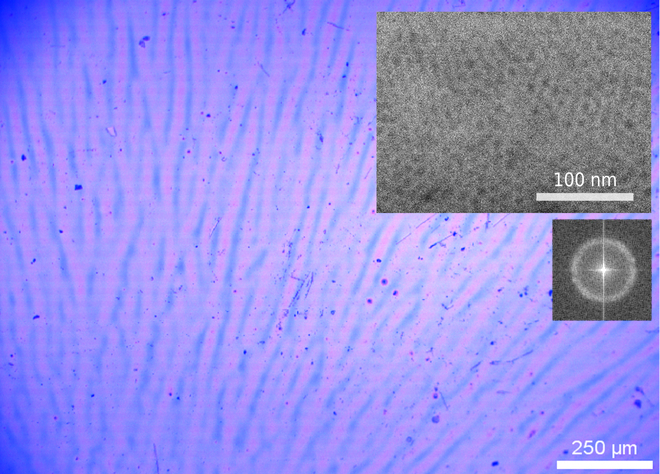
\includegraphics[width=\textwidth]{Imagenes/Si_BF127-Combinada.jpg}
	   		\end{subfigure}
			 \caption[Microscopía óptica \pdmF tratamiento en medio alcalino.]{Microscopías ópticas para Alc\pdmF. Izquierda: sobre sustrato de Au. Derecha: sobre sustrato de Si. En los respectivos recuadros se observa el detalle por MEB junto a la transformada de Fourier (sobre silicio) del arreglo nanoporoso.}
			 \label{fig:Microscopia_F127_basico}	
		     \end{figure}

		%Microscopia CTAB
			\begin{figure}
 	   	    \begin{subfigure}{0.495\textwidth}
	       	\includegraphics[width=\textwidth]{Imagenes/Au_BCTAB-Combinada.jpg}
	   		\end{subfigure}
	   		\begin{subfigure}{0.495\textwidth}
	   	    \includegraphics[width=\textwidth]{Imagenes/Si_BCTAB-Combinada.jpg}
	   		\end{subfigure}
			 \caption[Microscopía óptica \pdmC tratamiento en medio alcalino.]{Microscopías ópticas para Alc\pdmC\space sintetizadas por el tratamiento de condensación y extracción en medio alcalino. Izquierda: sobre sustrato de Au. Derecha: sobre sustrato de Si.}
			 \label{fig:Microscopia_CTAB_basico}	
		     \end{figure}		

		%Elipso F127
			\begin{figure}
		  	\begin{subfigure}{0.495\textwidth}
		  	\includegraphics[width=\textwidth]{Graficos/SI_F127_basico_EPA.pdf}
			\caption[Elipsoporsimetría \pdmF\space tratamiento básico.]{Isoterma de adsorción/desorción de agua realizada por PEA para una \pdmF.}
			\label{fig:F127_basico_EPA}
			\end{subfigure}
			\begin{subfigure}{0.495\textwidth}
		  	\includegraphics[width=\textwidth]{Graficos/SI_F127_basico_PSD.pdf}
			\caption{Distribución de tamaño de poro y cuello.\\ }
			\label{fig:F127_basico_PSD}
			\end{subfigure}
			\caption[Elipsoporosimetría \pdmF\space tratamiento básico.]{Resultados de elipsoporosimetría ambiental para una Alc\pdmF.}
			\end{figure}
		
		%Elipso CTAB
			\begin{figure}
		  	\begin{subfigure}{0.495\textwidth}
		  	\includegraphics[width=\textwidth]{Graficos/SI_CTAB_basico_EPA.pdf}
			\caption[Elipsoporsimetría \pdmC\space tratamiento básico.]{Isoterma de adosroción/desorción de agua realizada por PEA para una Alc\pdmC.}
			\label{fig:CTAB_basico_EPA}
			\end{subfigure}
			\begin{subfigure}{0.495\textwidth}
		  	\includegraphics[width=\textwidth]{Graficos/SI_CTAB_basico_PSD.pdf}
			\caption{Distribución de tamaño de poro y cuello.\\ }
			\label{fig:CTAB_basico_PSD}
			\end{subfigure}
			\caption[Elipsoporosimetría \pdmC\space tratamiento básico.]{Resultados de elipsoporosimetría ambiental para una Alc\pdmC.}
			\end{figure}	
		
		%FTIR F127
			\begin{figure}
			\centering
			\includegraphics[width=0.75\textwidth]{Graficos/IR_F127_basico.pdf}
			\caption[FTIR \pdmF\space tratamiento básico.]{Espectro de absorción en el IR para una Alc\pdmF\space antes y después de extraer el surfactante. Obsérvese la ausencia de hombro en la región 1250-\SI{1100}{\cm^{-1}}, la cual es típica de sistemas de SiO$_2$ mesoestrucuturas.}
			\label{fig:IR_F127_basico}
			\end{figure}

		%FTIR CTAB	

			\begin{figure}
			\centering
			\includegraphics[width=0.75\textwidth]{Graficos/IR_CTAB_basico.pdf}
			\caption[FTIR \pdmC\space tratamiento básico.]{Espectro de absorción en el IR para una Alc\pdmC\space antes y después de extraer el surfactante. Obsérvese la ausencia de hombro en la región 1250-\SI{1100}{\cm^{-1}}, la cual es típica de sistemas de SiO$_2$ mesoestrucuturas.}
			\label{fig:IR_CTAB_basico}
		    \end{figure}
		
		\clearpage\subsection*{Figuras correspondientes al capítulo \ref{chap:Electroquimica}}

		  	 \begin{figure}[ht]	
					\begin{subfigure}[t]{0.495\textwidth}
			 	    \includegraphics[width=\textwidth]{Graficos/aptesfecn-10mM.pdf}
			        \caption{Respuesta utilizando como sonda negativa \ferroferri\space \SI{1}{\milli\Molar}.}
			        \label{fig:aptes10mM-vc-fe}
			        \end{subfigure}
			        \begin{subfigure}[t]{0.495\textwidth}
			 	    \includegraphics[width=\textwidth]{Graficos/aptesru-10mM.pdf}
			        \caption{Respuesta utilizando como sonda positiva \aminorutenio\space \SI{1}{\milli\Molar}.}
			        \label{fig:aptes10mM-vc-ru}
			        \end{subfigure}
			        \caption[Voltagramas de \pdmZ$^P_3$ con \aminorutenio\space y \ferroferri]{Respuesta comparativa entre \pdmZ\space funcionalizadas con APTES \SI{10}{\milli\Molar} y sin funcionalizar. Para cada experimento se tomaron más de 90 voltagramas consecutivos en KCl \SI{100}{\milli\Molar} a \SI{50}{\milli\volt\per\second}.}
			        \label{fig:aptes10mM-vc}
			      	\end{figure}

		\null
		\vfill		

%Restituye el estilo
\let\thispagestyle=\originalstyle